\documentclass[a4paper,10pt]{article}
\usepackage[utf8]{inputenc}
\usepackage{amsmath}
\usepackage{graphicx}
\usepackage{subcaption}
\usepackage{hyperref}


%\usepackage{framed}
%\usepackage{amsfonts}

%\usepackage{amssymb}
%\setlength{\parindent}{0pt}

\usepackage{diagbox} %Allow diagonally split cell in latex

\usepackage{float}
\usepackage{epstopdf}
\usepackage{pdfpages} %Utility to include pdf documents into the report, used to include datasheets in appendices.

\usepackage{tikz}
\usepackage{circuitikz}

%Following mess allows for creating IC's in tikz..
\usepackage{mathtools}
\usetikzlibrary{calc,arrows} 
\makeatletter
\pgfdeclareshape{circuit}{
  \savedanchor\northeast{
    \pgfmathsetlength\pgf@x{\pgfshapeminwidth}
    \pgfmathsetlength\pgf@y{\pgfshapeminheight}
    \pgf@x=0.5\pgf@x
    \pgf@y=0.5\pgf@y}
  \savedanchor\southwest{
    \pgfmathsetlength\pgf@x{\pgfshapeminwidth}
    \pgfmathsetlength\pgf@y{\pgfshapeminheight}
    \pgf@x=-0.5\pgf@x
    \pgf@y=-0.45\pgf@y}
  \inheritanchorborder[from=rectangle]
  \anchor{center}{\pgfpointorigin}
  \anchor{north}{\northeast \pgf@x=0pt}
  \anchor{east}{\northeast \pgf@y=0pt}
  \anchor{south}{\southwest \pgf@x=0pt}
  \anchor{west}{\southwest \pgf@y=0pt}
  \anchor{north east}{\northeast}
  \anchor{north west}{\northeast \pgf@x=-\pgf@x}
  \anchor{south west}{\southwest}
  \anchor{south east}{\southwest \pgf@x=-\pgf@x}
  \anchor{text}{
    \pgfpointorigin
    \advance\pgf@x by -.5\wd\pgfnodeparttextbox
    \advance\pgf@y by -0.1875\ht\pgfnodeparttextbox
    \advance\pgf@y by +.5\dp\pgfnodeparttextbox}
\anchor{ina}{
  \pgf@process{\northeast}
  \pgf@x=-1\pgf@x
  \pgf@y=0.5\pgf@y}
\anchor{outa}{
  \pgf@process{\northeast}
  \pgf@y=0.5\pgf@y}
\anchor{outb}{
  \pgf@process{\northeast}
  \pgf@y=0.09999999999999998\pgf@y}
\anchor{outc}{
  \pgf@process{\northeast}
  \pgf@y=-0.3\pgf@y}
\anchor{inb}{
  \pgf@process{\northeast}
  \pgf@x=-1\pgf@x
  \pgf@y=0.09999999999999998\pgf@y}
\anchor{outd}{
  \pgf@process{\northeast}
  \pgf@y=-0.7000000000000001\pgf@y}
\backgroundpath{
  \pgfpathrectanglecorners{\southwest}{\northeast}
  \begingroup
    \tikzset{labels}
    \tikz@textfont
  \endgroup}}
\tikzset{add font/.code={\expandafter\def\expandafter\tikz@textfont\expandafter{\tikz@textfont#1}}}
\tikzset{labels/.style={font=\sffamily\scriptsize}}
\tikzset{every circuit node/.style={draw,minimum width=2cm,minimum height=2.5cm,very thick,inner sep=1mm,outer sep=0pt,cap=round,add font=\sffamily\bfseries}}
\makeatother
\DeclarePairedDelimiter\ceil{\lceil}{\rceil}
\DeclarePairedDelimiter\floor{\lfloor}{\rfloor}
\newcount\colveccount
\newcommand*\colvec[1]{
        \global\colveccount#1
        \begin{pmatrix}
        \colvecnext
}
\def\colvecnext#1{
        #1
        \global\advance\colveccount-1
        \ifnum\colveccount>0
                \\
                \expandafter\colvecnext
        \else
                \end{pmatrix}
        \fi
}

\usepackage{todonotes}
%opening
\title{Brick Sorter}
\author{Thomas Søndergaard Christensen, Keerthikan Ratnarajah}
\date{dd/mm/yyyy}

\begin{document}
\begin{titlepage}
\begin{center}

\textsc{\LARGE University of Southern Denmark}\\[1.5cm]
\textsc{\large Robot Electronics - Mandatory Exercise 3}\\[0.5cm]
\vfill
\hrule ~\\[0.3cm]
{ \huge \bfseries Rotating LED Display\\[0.4cm] }
\hrule ~\\[1.5cm]
\vfill

% Author and supervisor
\begin{minipage}[t]{.49\textwidth}
\begin{flushleft} \large
\textbf{Author:}\\
100589 Thomas S. Christensen \\
020692 Keerthikan Ratnarajah\\
\end{flushleft}
\end{minipage}
\begin{minipage}[t]{.49\textwidth}
\begin{flushright} \large
\textbf{Supervisors:} \\
Cand. Polyt. Richard Beck\\
Ph. D. Jørgen Christian Larsen
\end{flushright}
\end{minipage}

\vspace{1.2cm}
Date: 23-12-2015

\end{center}
\end{titlepage}

\newpage
\tableofcontents
\newpage
\listoffigures
\listoftables
\listoftodos
\clearpage
\newpage

\section{LED Driver}
The brick sorter relies on the varying reflective properties of different colours. Using a variety of different colour LEDs will enable the sorter to detect different colour bricks. This section will describe in detail the decisions made in designing the circuit used for the LEDs and the photo diode as well as presenting the code responsible for driving the LEDs. 

\subsection{Circuit Design}
\begin{figure}[h!]
	\begin{center}
		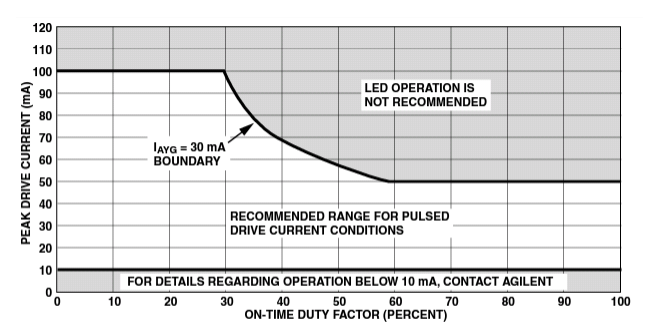
\includegraphics[width=\linewidth]{images/overdrive}
	\end{center}
	\caption{The white region denotes the area in which the LED can safely be driven.}
	\label{fig:overdrive}
\end{figure}
The switching of the LEDs is done using bipolar junction transistors (BJTs). The BJTs are wired as a simple switching circuit as in figure \ref{circ:ledswitch}. $V_{\text{c}}$, the switching signal, will be generated using an FPGA.
In order to achieve the highest possible light intensity from the LEDs they will be overdriven. Figure \ref{fig:overdrive} is an excerpt from \cite{avago}. This graph shows that the LEDs can be safely driven at 100mA so long as the duty cycle of $V_{\text{c}}$ does not exceed 30\%. Driving the LEDs at 100mA implies that $I_c=100\text{mA}$. 

For a BJT:
\begin{eqnarray}
I_c=&I_b\cdot h_{\text{FE}}\\
I_b=&\frac{V_{\text{c}}-V_{be}}{R_1}
\end{eqnarray}
Looking at the datasheet of the BC547b the dc current gain of this transistor is found to be
\begin{eqnarray}
	h_{\text{FE}}=200 \Rightarrow I_b = 0.5\text{mA}
\end{eqnarray}
Lastly, according to figure \ref{fig:vbe} from the datasheet of the BC547b, when $I_c = 100$mA $V_{be}=0.8$v.
Since the BJT is used as a switch it is desirable that it is driven to saturation quickly to avoid dissipating power in the component. Therefore, $I_b$ is doubled and 
\begin{eqnarray}
	R_1 = \frac{V_{\text{c}}-V_{be}}{I_b\cdot 2} = 2.5\text{k}\Omega
\end{eqnarray}

\begin{figure}[h!]
	\centering
	\begin{subfigure}[b]{.48\linewidth}
		\begin{circuitikz}
			\draw (0,0) 
			node[npn](npn1){}
			(npn1.base) ++(-2,0) node[name=r1left]{}
			to[R=$R_1$,o-,i=$I_b$] ++(2,0) ++(-2,0)node[left]{$V_{\text{c}}$}
			(npn1.base) ++(0.75,0) node[right]{BC547b}
			(npn1.emitter) 
			node[ground](GND){}
			(npn1.collector) ++(0,4) node[name=d_top]{}
			to[D=$LED$,o-]++(0,-2) 
			to[R=$R_2$,i=$I_c$]++(0,-2)
			(d_top) node[above]{$V_{cc}$}
			;\end{circuitikz}
		\caption{Switching circuit for single LED}
		\label{circ:ledswitch}
	\end{subfigure}
	\begin{subfigure}[b]{.48\linewidth}
		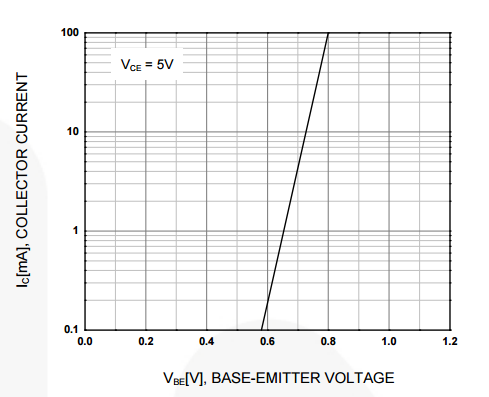
\includegraphics[width=\linewidth]{images/vbe}
		\caption{Graph of $I_c$ as a function of $V_be$.}
		\label{fig:vbe}
	\end{subfigure}
	\caption{(a)LED Circuit, three of these are combined to drive the red, green and blue LEDs used in this application. (b) Graph from the datasheet of the BC547p showing the correlation between collector current and base-emitter voltage.}
\end{figure}
\begin{figure}[h!]
	\begin{center}
		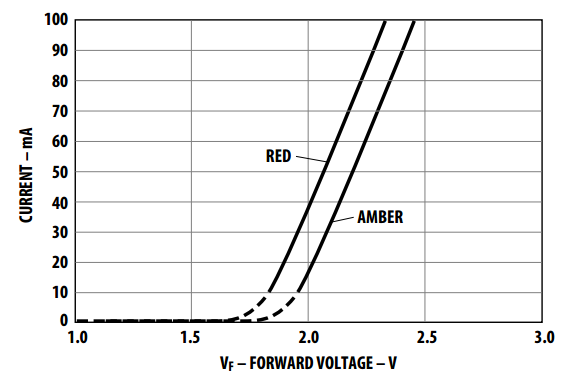
\includegraphics[width=0.75\linewidth]{images/redvd}
	\end{center}
	\caption{Current as a function of forward voltage for the red diode.}
	\label{fig:ledcurrent}
\end{figure}
Finding $R_2$ is done using the datasheets of the LEDs. figure \ref{fig:ledcurrent} shows the correlation between the voltage drop across the diode and the current through the diode.
According to these figures the red LED will have a voltage drop $V_d = 2.3$v and the green and blue LEDs will $V_d = 4$v. This results in 
\begin{eqnarray}
	R_{2\_\text{red}}=& \frac{V_{cc}-V_d}{I_c} &= 97\Omega \\
	R_{2\_\text{green}}=&R_{2\_\text{blue}} = \frac{V_{cc}-V_d}{I_c} &= 80\Omega
\end{eqnarray}

This next part of the circuit is responsible for detecting the reflected light and amplify the signal generated by the photodiode such that it can be processed by the ADC. A diagram of the circuit used can be seen in figure \ref{circ:unfiltered}.
The output voltage of this circuit is determined by:
\begin{eqnarray}
	V_{\text{out}}=&I_{\text{in}}\cdot R_f\\
	R_f =& R_1+R_{\text{pot}}
\end{eqnarray}
When an LED is flashed onto a same-coloured brick, the output of the op-amp is expected to be $V_{\text{out}} = V_{\text{sat}}$, the saturation voltage. By experimentation this was found to be $V_{\text{sat}}=3.78$v.

$I_{\text{in}}$ was determined by making the circuit as seen in figure \ref{circ:iinmeasure}. By reflecting the light from the LEDs off of the bricks and onto the photodiode, a current is induced in the circuit and a voltage drop can be measured across the 1k$\Omega$ resistor the maximum current to be expected generated from the photodiode was found to be $I_{\text{in}}=10\mu$A.
\begin{figure}[h!]
	\centering
	\begin{circuitikz}
		\draw(0,0) 
			to[short] ++(2,0)
				to[R=1k$\Omega$] ++(0,-2)
					to[short] ++(-2,0) 
						to[pD] ++(0,2) coordinate(d_right)
			(d_right) ++(-1.5,0) to[short,-o] ++(-1,0)
			(d_right) ++(-1.5,0) to[lamp] ++(0,-2)
				to[short,-o] ++(-1,0)
	;\end{circuitikz}
	\caption{Circuit used for measuring the max current expected to be generated from the photo diode when in operation.}
	\label{circ:iinmeasure}
\end{figure}

This results in $R_f=378\text{k}\Omega$, however, it was found that applying this resistor causes the blue brick to also saturate the op amp when shining the green LED. Additionally, when mounting the LED assembly to the acrylic slide, the slide itself was found to enlarge $I_{\text{in}}$ by a significant margin. Due to these factors $R_f$ was finally dimensioned using a 1M$\Omega$ potentiometer. \todo{And final value is?!}

\begin{figure}[h!]
  	\centering
	\begin{subfigure}[b]{.49\linewidth}
		\resizebox{\linewidth}{!}{
			\begin{circuitikz}
				\draw(0,0) 
					node[op amp] (opamp) {}
				(opamp.-) ++(-2,-1) 
					node[ground]{} to[short] ++(0,1)
						to[pD] (opamp.-)
				(opamp.-) to[short] ++(0,1) coordinate(capleft)
					to[R=$R_1$] ++(2,0)
						to[vR=$R_\text{pot}$] ++(2,0) coordinate(pot)
				(opamp.out) -| (pot) coordinate(conn)
					to[short] (pot)
				(opamp.+) to[short] ++(0,-0.5)
					node[ground]{}
			;\end{circuitikz}
		}
		\caption{Unfiltered version.}
		\label{circ:unfiltered}		
	\end{subfigure}
	\begin{subfigure}[b]{.49\linewidth}
		\resizebox{\linewidth}{!}{
			\begin{circuitikz}
				\draw(0,0) 
				node[op amp] (opamp) {}
				(opamp.-) ++(-2,-1) 
				node[ground]{} to[short] ++(0,1)
				to[pD] (opamp.-)
				(opamp.-) to[short] ++(0,1) coordinate(capleft)
				to[R=$R_1$] ++(2,0)
				to[vR=$R_\text{pot}$] ++(2,0) coordinate(pot)
				(opamp.out) to[short] (opamp.out -| pot) coordinate(conn)
				to[short] (pot)
				(opamp.+) to[short] ++(0,-0.5)
				node[ground]{}
				(capleft) to[short] ++(0,1) coordinate(capleftup)
				to[C=$C_f$] (capleftup -| pot)
				to[short] (pot)
				;\end{circuitikz}
		}
		\caption{Filtered version.}
		\label{circ:filtered}
	\end{subfigure}
   	\caption{Photo diode amplifier circuit}
   	\label{circ:photodiode}
\end{figure}

Table \ref{tab:ledtable} shows the various responses of the photodiode when exposed to the different LEDs and bricks.

\begin{table}
	\centering
	\begin{tabular}{| c | c | c | c | c |}
		\hline
		\diagbox{LED}{BRICK}& R & G & B & A\\
		\hline
		R & 2.97 & 1.11 & 1.30 & 1.66\\
		\hline
		G & 1.71 & 3.34 & 2.81 & 2.49\\
		\hline
		B & 1.78 & 2.00 & 3.86 & 2.38\\
		\hline
	\end{tabular}
	\caption[Response from photodiode circuit.]{Response from photodiode circuit. Each colour LED; red, green and blue is flashed while each colour brick is used as the reflective surface.}
	\label{tab:ledtable}
\end{table}
\subsection{Circuit Testing}
In testing, a significant amount of oscillation appeared on the output of the op amp. See figure \ref{fig:oscillation}. To avoid issues when digitizing the signal with the ADC, it will be filtered by applying a compensation capacitor in parallel with $R_f$, see figure \ref{circ:filtered}.

\begin{figure}[h!]
	\centering
	\begin{subfigure}{\linewidth}
		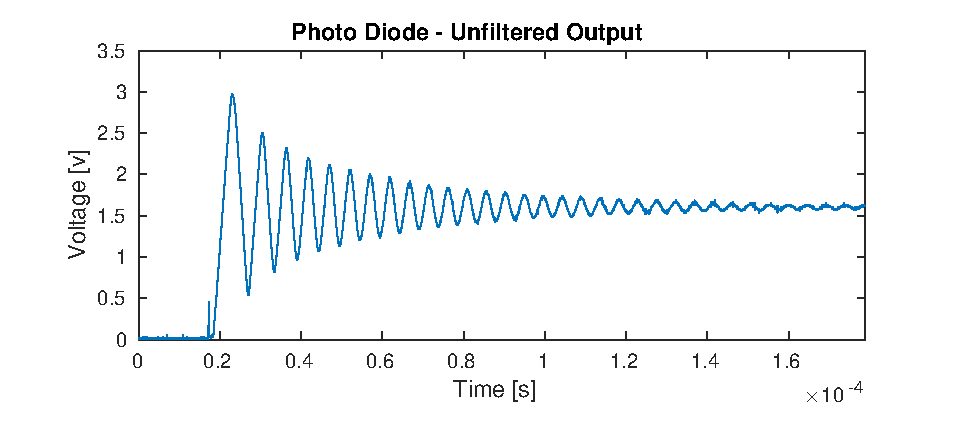
\includegraphics[width=\linewidth]{images/unfiltered}
		\caption{Unfiltered output.}
		\label{fig:oscillation}
	\end{subfigure}\\
	\begin{subfigure}{\linewidth}
		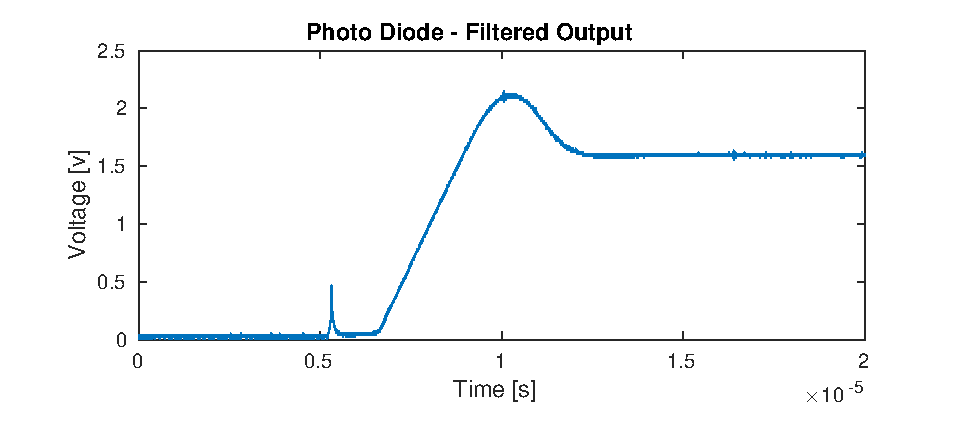
\includegraphics[width=\linewidth]{images/filtered}
		\caption{Filtered output.}
		\label{fig:nooscillation}
	\end{subfigure}
	\caption{Response of the photodiode amplifier circuit. Note the order of dimension difference on the timescale, (b) is stable within one period of (a).}
	\label{fig:photoresponse}
\end{figure}

 According to \cite{mec} the compensation capacitor is dimensioned using
\begin{equation}
	\label{eq:rcfilter}
	f_c=\frac{1}{2\pi R C}
\end{equation}
The oscillation happens at $\approx 138\text{kHz}$ and $R = R_f = 160\text{k}$ this results in 
$$C = 7.2\text{pF}$$ \todo{verify capacitor value}
The filtered signal can be seen in figure \ref{fig:nooscillation}. After filtering there is still a significant settling time, $T_{\text{s}}$, before the signal can be safely digitized. $T_{\text{s}}$ varies with the amplitude of the final signal, therefore a conservative time before sampling with the ADC must be set. 
On figure \ref{fig:settletime} it can be seen that the worst case settling time is an expected $T_{\text{s}}=12.65\mu$s.
\\
Later sources \cite{maxim} suggest that, in the case of dimensioning the compensation capacitor for a transimpedance amplifier, TIA, one should apply the following formula:
\begin{equation}
	c_f=\frac{1}{4\pi R_\text{F}f_\text{GBWP}}(1+\sqrt{1+8\pi R_\text{F}C_if_\text{GBWP}})
\end{equation}
Here, $f_\text{GBWP}$ is the unity gain band width of the op amp and $C_i$ is the capacitance of the photodiode. 
The resultant capacitance should result in the optimal value such that oscillation is minimized whilst not impeding on the performance of the op amp. In the case of the circuit of this design the capacitance should be:
\begin{gather}
	R_F = 165\text{k}\Omega \quad \text{,} \quad f_\text{GBWP}=0.7\text{MHz} \quad \text{,} \quad C_i=11\text{pF}\\
	c_f = 4.725 \text{pF}
\end{gather}
Using the value found by equation \ref{eq:rcfilter} would overcompensate the system and could potentially hinder the slew rate of the circuit. Since the entire reasoning behind dampening the oscillation in the first place was to decrease $T_\text{s}$, a 4.8pF, the nearest available size, capacitor was chosen as the compensation capacitor.  
\begin{figure}[h!]
	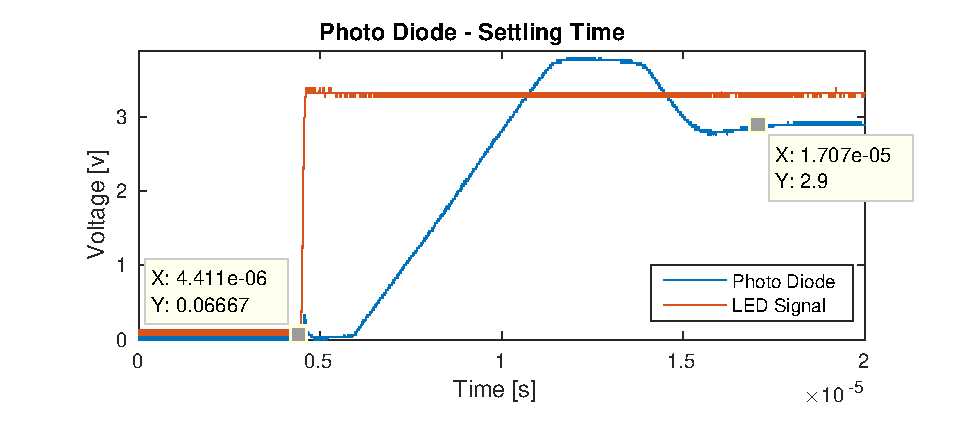
\includegraphics[width=\linewidth]{images/settle}
	\caption{Worst case settling time. When LED signal goes high, the photo diode is expected to have settled after $T_{\text{s}}=12.65\mu$s.}
	\label{fig:settletime}
\end{figure}

\subsection{LED Driver}
The LED driver is the VHDL component that contains the logic that determines which LED is on at any given time.
\begin{figure}[h!]
	\centering
	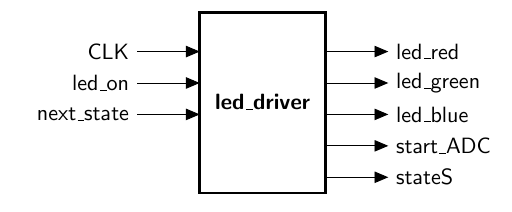
\includegraphics[scale=1]{images/LED_ent}
	\caption{heading}
	\label{fig:pinoutled}
\end{figure}
Only one LED is on at a time such that the reflection of each colour can be measured by the photodiode individually.
As mentioned in the previous section the LED has to be turned on for 13 $\mu$s such that output of the photodiode can settle such that the voltage is steady for the ADC conversion.
\subsection{Implementation of the LED driver}

The LED driver is implemented with 2 processes , \texttt{state\_changer} and \texttt{LED\_process}. 

\texttt{State\_changer} consists of a finite state machine, FSM, which has three states , \texttt{Red}, \texttt{Green}, \texttt{Blue} which each turn on their respective LED, and turn off the others.  The FSM start at \texttt{Red}.  At this state \texttt{led\_red} is set to high.\\

In \texttt{LED\_process}, \texttt{count} is incremented for each \texttt{rising\_edge} of \texttt{CLK}.  When \texttt{count} goes above 650, 13 $\mu$s have passed, and  \texttt{start\_ADC} is set high. 
\texttt{start\_ADC} is used to signal to the ADC component that a conversion is needed.
Once the conversion is completed, this will be signalled to the control module, see section \ref{sec:control}, which in turn will set \texttt{next\_state} high.
When \texttt{next\_state} goes high, \texttt{count} is reset, \texttt{start\_ADC} is set low  and the state machine progresses to the next state.
%% May have to remove LED_on.. Don't have to turn them off.. 

\newpage
\section{Power Supply}
This section will explain in detail the design of the power supply that was created to drive the various parts of the brick sorter. Three rails will be created, two using linear voltage regulators and one using a switching regulator. The power supply will be tested to verify that it conforms with the given performance requirements.
\subsection{Parts and Requirements}
The power supply described in this section is to have three voltage rails:
\begin{itemize}
	\item LEDs: 12v/1000mA.
	\item SERVO: 6v/1500mA.
	\item FPGA: 5v/1A, $\pm$\% max output voltage, min 80\% efficient.
\end{itemize}
The power supply itself is supplied with 15v. A list of components was provided in order to facilitate the design process. These are the main components of the power supply:
\begin{itemize}
	\item LM2574: Step-Down Switching Regulator. Datasheet \cite{lm2574}
	\item NCP7812TG: 12v Linear Voltage Regulator. Datasheet \cite{ncp7812}
	\item L7806cv: 6v Linear Voltage Regulator. Datasheet \cite{l7806}
\end{itemize}
Additionally, a PCB must be designed for the power supply.
\subsection{Design}
Since most of the components of the power supply are given, the task of design is mostly one of laying out the PCB. This is done by using Eagle\footnote{CadSoft EAGLE v7.4.0 Light Edition}. The schematics of the three different voltage rails can be seen in figure \ref{fig:psuschematic}.
The capacitors $C_3$ and $C_5$ are dimensioned according to the application circuit from their respective datasheet. They are omittable at low current operation or if the regulator is an appreciable distance from its power source. With no way of interpreting "appreciable distance" and operation being 1A and 1.5A for the 12v rail and the 6v rail respectively, it was decided to include them. Likewise, capacitors $C_4$ and $C_6$ serve to improve the transient response of the component.

The output and input of the linear voltage regulators is connected using a flyback diode. This is especially important on the 6V rail. This rail will be connected to the servomotor which, in a sense, is a coil, which can produce significant back electromotive force that could potentially damage the circuit.

The inherent inefficiency of linear voltage regulators gives cause to some thermal considerations, as any excess voltage is converted to heat. According to the datasheet, the NCP7812 has a junction-to-case thermal resistance $R_{\theta\text{JC}}=7.5^\circ\text{C/W}$. For the L7806, $R_{\theta\text{JC}}=5^\circ\text{C/W}$ See table \ref{tab:thermals} for an overview of the theoretical maximum operating temperature, $T_\text{max}$ with no heatsink. As can be seen the 12V rail would reach a maximum of 90$^\circ$C which is well below the maximum junction temperature of 125$^\circ$C listed in the datasheet, but well above what is considered pleasant to touch. To avoid burns while testing a heatsink is mounted. The 6V rail should not require a heatsink.

\begin{table}[h!]
	\centering
	\begin{tabular}{| c | c | c | c |}
		\hline
		Rail & Max curr. [A] & Max pow. [W] & $T_\text{max}$ [$^\circ$C] \\
		\hline
		12V  & 1.0 & 12 & 90 \\
		\hline
		6V   & 1.5 & 9 & 45\\
		\hline		
	\end{tabular}
	\caption[Maximum operating temperature]{Calculated maximum operating temperature of the 6V and 12V rails.}
	\label{tab:thermals}
\end{table}

\begin{figure}[h!]
	\begin{subfigure}{.48\linewidth}
		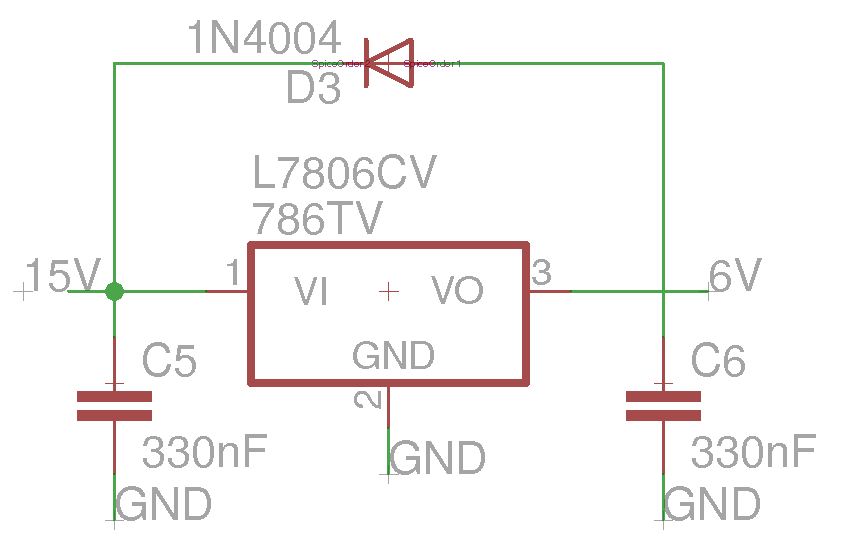
\includegraphics[width=\linewidth]{images/linear6v}
		\caption{Circuit for 6v rail.}
		\label{fig:psu6v}
	\end{subfigure}
	\begin{subfigure}{.48\linewidth}
		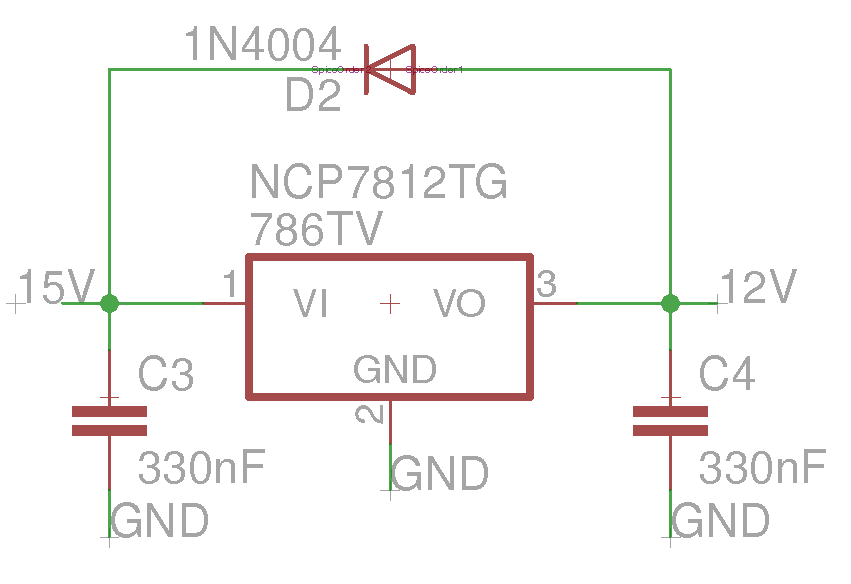
\includegraphics[width=\linewidth]{images/linear12v}
		\caption{Circuit for 12v rail.}
		\label{fig:psu12v}
	\end{subfigure}\\
	\begin{subfigure}{\linewidth}
		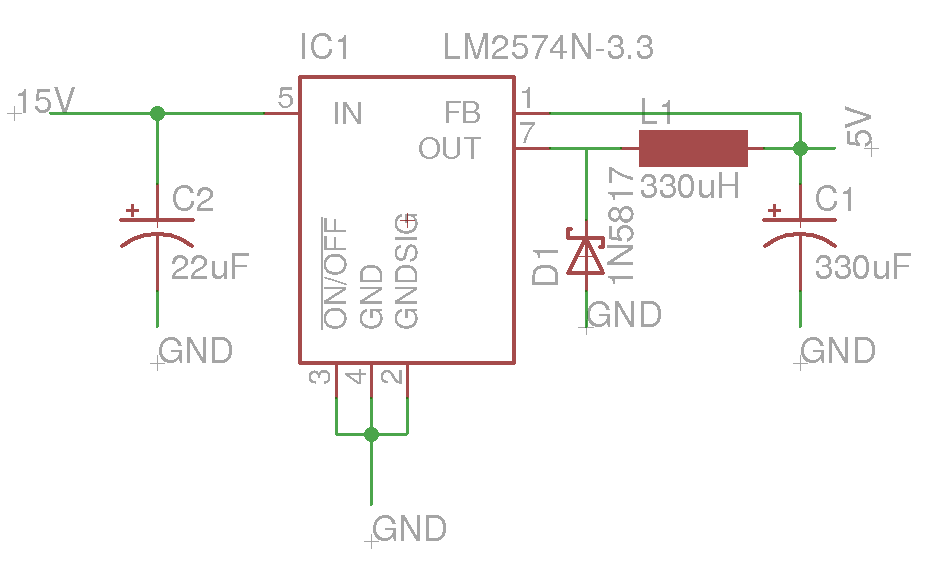
\includegraphics[width=\linewidth]{images/switch5v}
		\caption{Circuit for 5v rail.}
		\label{fig:psu5v}
	\end{subfigure}
	\caption{Schematics of the power supply.}
	\label{fig:psuschematic}
\end{figure}

The switching regulator in figure \ref{fig:psu5v} is designed as the typical applications design in the datasheet of the LM2574 \cite{lm2574}. This design is accompanied with a graph for dimensioning the size of the output inductance, $L_1$, see figure \ref{fig:inductorselect}. Since the IC will be supplied with 15V and a maximum load of 0.5A is required, the inductor necessary is 330$\mu$H. The value of the output capacitor, $C_1$ is determined according to 
\begin{eqnarray}
	C_\text{out}\geq&13300\frac{V_\text{in}(\text{MAX})}{V_\text{out}\cdot L(\mu\text{H})}(\mu\text{F})\\
	C_\text{out}\geq&13300\frac{15}{5\cdot 330} = 120.9(\mu\text{F})
\end{eqnarray} 
For this design, a 330$\mu$F capacitor is provided, which, while large, does fulfil the specification.
\begin{figure}[h!]
	\centering
	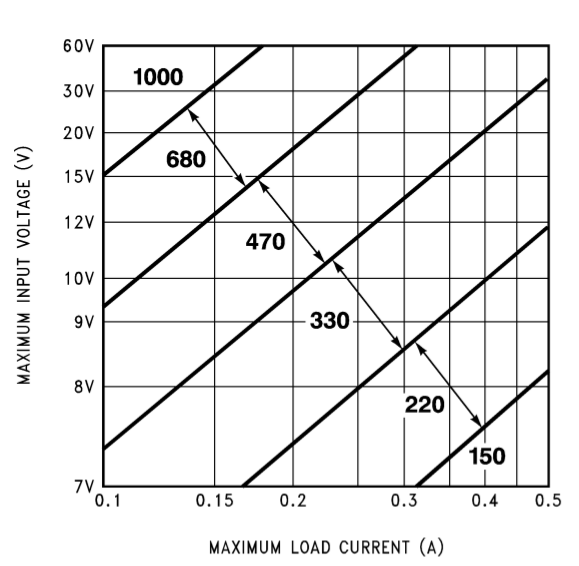
\includegraphics[width=.6\linewidth]{images/inductorselector}
	\caption{Graph showing the necessary inductance at various voltages and loads.}
	\label{fig:inductorselect}
\end{figure}
\\~\\

\subsection{Testing}
As previously mentioned the 5V rail must be at least 80\% efficient. However, according to the datasheet, the 5V version of the LM2574 is capable only of 77\% efficiency. Even though achieving the goal of 80\% efficiency will be difficult, the efficiency of this rail, as well as the others can still be tested and documented. Each rail will be tested for efficiency at 25\%, 50\%, 75\% and 100\% load. The results of this test can be seen in table \ref{tab:efficiency}. 
\begin{table}[h!]
	\centering
	\begin{tabular}{| c | c | c | c | c |}
		\hline
		Rail & Eff. 25\% & Eff. 50\% & Eff. 75\% & Eff. 100\% \\
		\hline
		12V  & 74.04 & 76.86 & 77.89 & 78.43\\
		\hline
		6V   & 37.89 & 38.95 & 39.31 & 39.45\\
		\hline		
		5V   & 75.75 & 76.19 & 76.34 & 77.24\\
		\hline
	\end{tabular}
	\caption[Power supply efficiency]{Efficiency of the various rails on the power supply.}
	\label{tab:efficiency}
\end{table}
As expected, the 5v rail peaks at $\approx77\%$ efficiency. The two rails controlled by linear voltage regulators clearly show the deficiencies of this technology. In the case of the 12V rail efficiency seems good, however it turns out that this efficiency is approximately equal to the relation between the input and output of the regulator, the same as for the 6V rail. The higher the difference between the input and output rails, the worse the efficiency. 
\newpage
\section{ADC}
The digital logic used to determine the color of a brick requires that the analog voltage is converted to a digital value. To this end, an analog to digital converter, ADC, is used. Specifically an MCP3008 \cite{mcp3008} which is a 10 bit ADC.
\subsection{The ADC: MCP3008}
As mentioned, the MCP3008 is an ADC, it is capable of converting an analog value ranging from 0 to V$_{\text{ref}}$ into a 10 bit value. It is rated to have a conversion rate of 200 ksps at V$_{\text{dd}} = 5$V. 

\begin{figure}[h!]
	\centering
	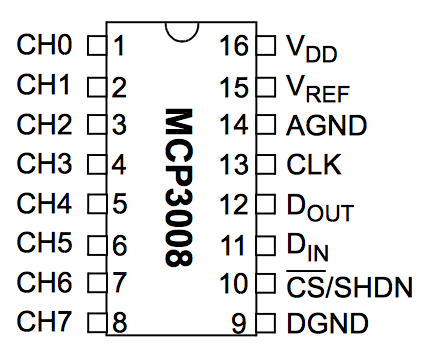
\includegraphics[scale = 0.5]{images/MPC3008.png}
	\caption{Pinout diagram of the MCP3008 ADC.}
	\label{fig:pinout}
\end{figure}
As can be seen on figure \ref{fig:pinout}, The chip is a 16 pin dip package. Pins 1 through 8 consist of eight seperate input ports for analog voltages. Pins 9 through 16 are, in descending order: V\textsubscript{dd}, V\textsubscript{ref}, AGND , CLK, \dout,  \din, \cs and GND. 
The ADC uses an SPI-based interface to communicate with the FPGA. For this communication four of the previously mentioned pins are utilized: CLK, \cs, \dout, \din. The purpose of these four pins will be explained in more detail in the following paragraphs


\paragraph{CLK:}
This pin, perhaps not surprisingly, will receive the clock signal. According to the datasheet the max frequency for communication is 3.57 MHz, which is provideded by the FPGA at that port.

\paragraph{D$_\text{in}$:}
This is the input port which the FPGA sends the five init bits to. 
bit five is the start bit ,  bit four determines whether the system should perform a single ended or differential conversion. 
Single ended conversion converts the input from one port and differential conversion converts the difference between two ports. 
The three LSBs determines from which input port the conversion should be done.
The init bits can be sent at either the rising, or the falling edge of the clock.\\

In this application, only one value needs to be converted, namely the signal from the photo diode amplifier. 
This signal is connected to CH0.
Additionally conversion will always be single ended, therefore the init bits will always be of the same form: "11000".

\paragraph{D$_\text{out}$:}
This is the output port from which the FPGA reads the converted signal as a 10 bit binary number. 
When a conversion has been performed,  the first bit which will be read from \dout will be the a null bit.
Following the null bit are the 10 bits outputted from MSB to LSB. 
\dout will stay undefined until the init bits have been provided on \din and the sample and hold period has passed. 
The sample and hold period is 1.5 clock cycles as per the datasheet. 
Due to this sample and hold period, the output is given on the inverse clock edge as the init bits were received.
It is custom to send init bits on the falling edge and read the output on the rising edge.


\paragraph{$\overline{\textbf{CS}}:$}
This pin acts as chip select. It is used to initiate communication between the ADC and FPGA.
Pulling \cs low initiates communication mode. Pulling \cs high ends the communication and puts the ADC in low-power standby mode.  
\cs must be toggled between each new conversion. 
 
\begin{figure}[h!]
	\centering
	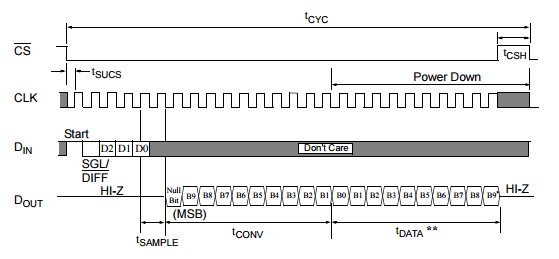
\includegraphics[width=\linewidth]{images/timing}
	\caption{Diagram showing the timings of a single communication.}
	\label{fig:timing}
\end{figure}

The entire communication process done to read a single conversion is depicted in figure \ref{fig:timing}. As can be seen, when \cs goes low, \din receives the five init bits. The sample and hold time is passed and a NULL bit followed by the result of the conversion is output on \dout. Throughout the period t$_\text{data}$ the chip is powering down and \dout reaches a high impedance state.
\subsection{Implementation of communication}
The communication between the MPC3008 and the FPGA is implemented as a VHDL component named ADC. 
The communication is implemented based on the timing diagram as showed in \ref{fig:timing}.  

\begin{figure}[h!]
	\centering
	\centerline{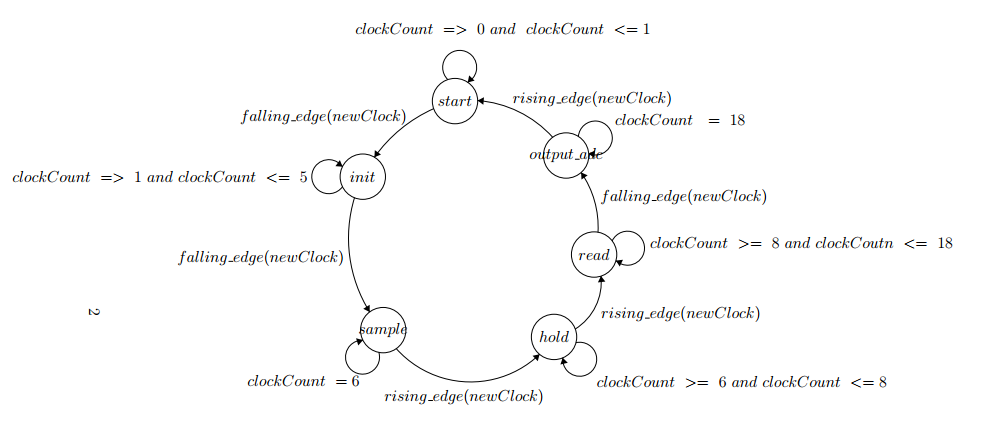
\includegraphics[width=18cm]{images/statemachine}}
	\caption{Program flow of the ADC component.}
	\label{fig:statemachine}
\end{figure}

As the MCP3008 operates at a clock frequency lower than what the FPGA provides. 
A process named \texttt{prescaler01} is designed to downscale the 50MHz external clock to the 3.57MHz required by the ADC. 
The downscaled clock is routed to \texttt{newClock}.


The process \texttt{ADC\_states}, increments \texttt{clockCount} for each rising edge on \texttt{newClock}.
This process detects both the falling and rising edges of \texttt{newClock}.

The progression of the state machine is based on the value of \texttt{clockCount}. 
This progression can be seen in figure \ref{fig:statemachine} and is explained below.\\

When \texttt{clockCount} is:
\begin{itemize}
	\item \textbf{0-1:} on the \texttt{falling\_edge} of \texttt{newClock}, \cs is set high, \texttt{MOSI} is set low and \texttt{read\_adc} is set low, signalling that conversion is not yet complete.\\
	\item \textbf{1-5:}on the \texttt{falling\_edge} of \texttt{newClock}, \cs is set low and the init bits are transmitted on \texttt{MOSI}, MSB first.
	\item \textbf{6:} on the \texttt{falling\_edge} of \texttt{newClock}, \texttt{MOSI} is set low. At this state MCP3008 starts sample and hold.
	\item \textbf{6-8:} on the \texttt{falling\_edge} of \texttt{newClock}, \texttt{MOSI} is kept low while the conversion is running. At \texttt{clockCount}=8 the MCP3008 outputs the NULL bit.
	\item \textbf{8-18:} on the \texttt{falling\_edge} of \texttt{newClock}, all 10 bits of the conversion are shifted from \texttt{MISO} into RX, a \texttt{std\_logic\_vector} containing the result of the conversion.
	\item \textbf{18:} on the \texttt{falling\_edge} of \texttt{newClock}, \texttt{read\_adc} is set high, signalling that conversion is complete and the result is ready.
	\item \textbf{19:} on the \texttt{falling\_edge} of \texttt{newClock}, \texttt{clockCount} is reset and the process starts over.
\end{itemize}

The conversion itself takes up only 17 \texttt{rising\_edges}, however one \texttt{clockCount} is used to set \cs high  and one \texttt{clockCount} is used to make sure that it read the 10 bit value. 


%begin{figure}[htb]
%\centering
%\begin{tikzpicture}[font=\sffamily,>=triangle 45]
%  \node [shape=circuit] (item) at (0,0) {adc};
%  \draw [<-] (item.ina) node [anchor=west,labels] {} -- +(-1,0) node [anchor=east] {MISO};
%  \draw [->] (item.outa) node [anchor=east,labels] {} -- +(1,0) node [anchor=west] {MOSI};
%  \draw [->] (item.outb) node [anchor=east,labels] {} -- +(1,0) node [anchor=west] {CS};
%  \draw [->] (item.outc) node [anchor=east,labels] {} -- +(1,0) node [anchor=west] {SCLK};
%  \draw [<-] (item.inb) node [anchor=west,labels] {} -- +(-1,0) node [anchor=east] {CLK};
%  \draw [->] (item.outd) node [anchor=east,labels] {} -- +(1,0) node [anchor=west] {read\_adc};
%  \draw [<-] (item.inc) node [anchor=west,labels] {} -- +(-1,0) node [anchor=east] {start\_adc};
%  \draw [->] (item.oute) node [anchor=east,labels] {} -- +(1,0) node [anchor=west] {ADC\_value};
%\end{tikzpicture}
%\caption{Entity of adc}
%\end{figure}

\subsection{Logic Level Converters}
When supplied with 5V, the MCP3008 uses TTL for communication while the FPGA uses 3.3V CMOS. To protect the FPGA it is necessary to translate the logic high of TTL, $V_h=5V$, to logic high of CMOS, $V_h=3.3V$. In order to achieve this a simple circuit was utilized. See figure \ref{circ:logiclevel}. 

\begin{figure}
	\centering
	\begin{circuitikz}
		\draw(0,0)
			 node[above]{V$_\text{TTL}$}
				to[short,o-] ++(1,0)
					to[R=$R_1$] ++(2,0) node[circ]{} coordinate(junc)
							to[zDo=$D_1$] ++(0,-2)
								node[ground](){}
					(junc) to[short,-o] ++(1,0) node[above]{V$_\text{CMOS}$}
	;\end{circuitikz}
	\caption{Uni-directional logic level converter.}
\end{figure}  

\newpage
\section{Servo motor}
The purpose of the servo motor is control the "flipper", which separates the blocks. \\


A servo motor consist of an DC motor, potentiometer and a control circuit.  As the motor rotates, the resistance of the potentiometer changes,  which the the control circuit  uses and  regulate its movement and the direction based on it.   When the motor shaft is at the desired position the power supplied to the motor will be used stop the motor, such that it doesn't move away from the desired position. \\

The desired position is sent through the sense wire, (often the white wire). The position itself is defined as the duty cycle of the PWM signal that it is provided with, as seen on \ref{fig:Servo_position}. 
 
\begin{figure}[H]
\centering
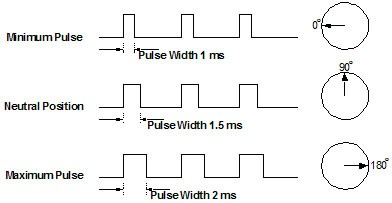
\includegraphics[scale=0.6]{images/servocontrol.jpg}
\label{fig:Servo_position}
%http://www.societyofrobots.com/actuators_servos.shtml
\end{figure}

\subsection{Interaction with Servo motor}
The control of the servo motor, is done using the FPGA with the entity named pwm. 

\begin{figure}[htb]
\centering
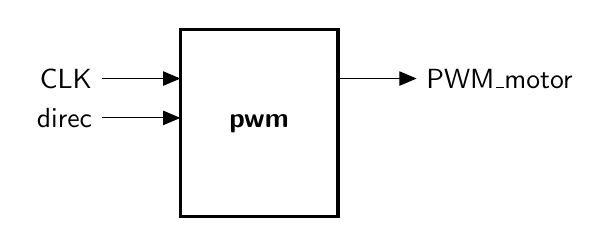
\begin{tikzpicture}[font=\sffamily,>=triangle 45]
  \node [shape=circuit] (item) at (0,0) {pwm};
  \draw [<-] (item.ina) node [anchor=west,labels] {} -- +(-1,0) node [anchor=east] {CLK};
  \draw [->] (item.outa) node [anchor=east,labels] {} -- +(1,0) node [anchor=west] {PWM\_motor};
  \draw [<-] (item.inb) node [anchor=west,labels] {} -- +(-1,0) node [anchor=east] {direc};
\end{tikzpicture}
\caption{Entity of pwm}
\end{figure}

\texttt{PWM\_motor} is connected to servo motor, and provides the PWM signal that sets the position of it. 
\texttt{direc} is an input signal, which tells the entity which direction the servo motor has to move to, and thereby deciding the duty cycle of the PWM signal. \texttt{CLK} is the clock frequency of the FPGA. \\

The component has only one process, that generates 3 different pwm signals based on the value of \texttt{direc}. If \texttt{direc} is "11" it moves to the right, if it is "00" it moves to the left, and if it has  other value it will stay neutral . \\


The period of the pwm signal of \texttt{PWM\_motor} is set to  20 ms, which the servo motors requires. 
For each  \texttt{rising\_edge} of the \texttt{CLK} a variable named \texttt{count} is incremented.  To make the motor move to left, will \texttt{PWM\_motor} stay zero until \texttt{count} is below 950000 and when it above 950000  and below 1000000 it will stay high, as 50000 \texttt{rising\_edge} equate to 1 ms. When count has reached 1000000 will it be reset again. \\





\newpage
\section{Control}
This section will explain in detail the code that combines the functionality of the ADC, LEDs and uTosNet(?)
\newpage
\begin{thebibliography}{11}
	\bibitem{mec}
		Sedra, Adel S., Smith, Kenneth C. Microelectronic Circuits, 3rd Ed. 1991, P. 630-632.
	\bibitem{avago}
		Avago Technologies. Pulsed Operating Ranges for AllnGaP LEDs vs. Projected Long Term Light Output Performance, Application Brief I-024, 2010
	\bibitem{lm2574}
		Texas Instruments. LM2574. 2013. http://docs-europe.electrocomponents.com/webdocs/0780/0900766b80780102.pdf
	\bibitem{maxim}
		maxim integrated. Stabilize Your Transimpedance Amplifier, Application Note 5129. 2012.
	\bibitem{mcp3008}
		Microchip Technology inc. MCP3004/3008. 2008. http://ww1.microchip.com/downloads/en/DeviceDoc/21295d.pdf
\end{thebibliography}

\newpage
\appendix
%\input{appendix/datasheet}

\end{document}